\documentclass[a4paper,10pt]{report}

\usepackage[utf8]{inputenc}
\usepackage{hyperref}
\usepackage{graphicx}
\usepackage{color}
\usepackage{array}
\usepackage{eurosans}

% Title Page
\title{Bicing}
\author{\textit{\textbf{Tomas Barton}} and \textit{\textbf{Mauro Donadeo}}}


\begin{document}
\maketitle

% \begin{abstract}
% \end{abstract}

\chapter{Introduction}
The aim of this project is to provide an program which would help the provider of local bicing service\footnote{Bicing Barcelona -- \url{http://www.bicing.com}} with distribution of bikes to approach to an ideal state, when each user of this service would find a bike when he needs it. 

\section{About Bicing}
The Bicing project is quite new in Barcelona (started in 2007\cite{bicingw}), but after few months it became very popular. Owner of a special card, which can be purchased for 30~\euro \, per year, can rent a bike from a station for free, if he returns this bike to some station in a half an hour. Otherwise he pays a few cents for each hour until the bike is returned. 

\begin{figure}[ht]
\begin{center}
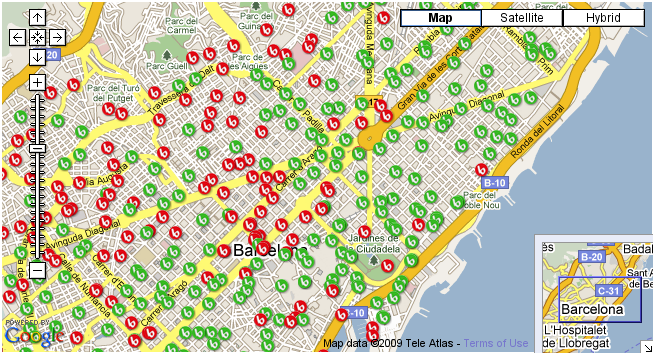
\includegraphics[width=\textwidth]{images/bicing_map.png}
\caption{Map of bicing stations in Barcelona -- red stations are without bikes}
\label{img:bicing_map}
\end{center}
\end{figure}

Nowadays there are more than 400\footnote{418 stations at 12 October 2009} bike stations in Barcelona, the highest concentration of bike stations is of course in centre of city. Usually each station has from 20 up to 30 stands for bikes. In the very center they are placed quite close to each other.

\section{Our task}
With usage of \textbf{\textsl{F}} vans we are supposed to optimize distribution of bikes, so that as many customers as possible will find a disposable bike at time when they need it.

Implementation has been done in Java, we took advantage of AIMA framework\cite{aima}, which contains most of algorithms commonly used for  searching state space.

\section{Complexity of problem}
As long as we have to search just for solution of this problem for upcoming hour, size of state space is significantly reduced. When we display all possible states of this problem as a n-ary tree, we get not really deep tree -- this is exactly the number of maximum moves we can do and that is \textbf{\textsl{F}}, but this tree can have a huge branching factor. 


\chapter{Implementation}
\section{State representation} 
Each state must contain information about distribution of bikes over all stations. So that we have to keep:
\begin{itemize}
\item current number of bikes at the station
\item number of bikes that is going to be at station in an hour 
\item moves how to reach this state (from empty state)
\end{itemize}
These information are different for each state, moreover we have other information which we need but they are same for every state:
\begin{itemize}
 \item number of stations
 \item coordinates of stations
 \item expected demand for bikes in upcoming hour
\end{itemize}


\section{Operators}

\begin{description}
 \item[moveBikes] simply moves given number of bikes from one station to another
\item[doubleMove] loads \( a + b \) bikes at one station and unload \(a\) bikes at first station and \(b\) bikes at second station
\item[changeMove] alter number of bikes or destination of this move
\item[removeMove] deletes specified move
 \end{description}

\section{Heuristic functions}


\clearpage
\begin{thebibliography}{9}
\bibitem{aima}{\em Stuart Russell and Peter Norvig:}{\bf Artificial Intelligence: A Modern Approach}
		\url{http://aima.cs.berkeley.edu/} \\
		{Downloaded java implementation of algorithms (AIMA framework) from repository \url{http://code.google.com/p/aima-java/} by Ravi Mohan. Date of publication: October 3, 2009. \\
		Date retrieved: October 12, 2009. }
\bibitem{bicingw}{\em Wikipedia: }{\bf Bicing}
\url{http://en.wikipedia.org/wiki/Bicing}\\
{Date visited: October 27, 2009}


\end{thebibliography}



\end{document}          
